%!TEX root = ../../report.tex

\subsection{CityEngine \cite{Parish2001} \cite{Muller2006}}
\label{sub:cityengine}

It's a three-dimensional (3D) modeling software developed by Procedural Inc. (now part of the Esri R&D Center). It's specialized in the generation of 3D urban environments. With the procedural modeling approach, CityEngine enables an efficient creation of detailed and large-scale 3D city models with a lot of control from the user. 

\subsubsection{RoadNetwork} % (fold)
\label{ssub:roadnetwork1}


The first part to procedurally generate a city is to create a road network to become a backbone of the city and provide an overall structure. For that, CityEngine receives as input maps such as land-water boundaries and population
density. From that input a network of highways is created to connect the areas off high density population, and small roads connect to the highways.
This growth process continues until the average area of each lot is the desired one. The system have a default value, bat it can be set by the user to a different one.

To implement this growth process, it's used an L-System, that computes the road network.


\begin{figure}[htbp]
  \centering
  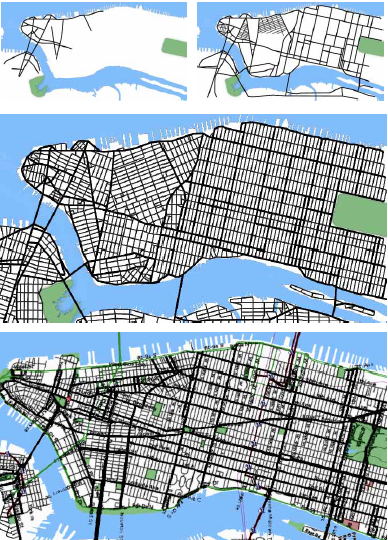
\includegraphics[width=0.5\textwidth]{img/Procedural-Modeling-of-Cities/Capturar.png}
  \caption{Road Map growth}
  \label{fig:city}
\end{figure}

The Figure~\ref{fig:city} shows the evolution of this process in a map of Manhattan. The first two on the top shows the process in different phases during the process, the middle line is the result of the process and the bottom line is the real map of Manhattan for comparison.

% subsubsection roadnetwork (end)Road Network

\subsubsection{Buildings} % (fold)
\label{ssub:buildings1}

To implement the generation of buildings, they created the CGA Shape.

CGA Shape is a Shape Grammar that was introduced by Pascal Muller, Peter Wonka and others, in a paper called ``Procedural Modeling of Buildings''\cite{Parish2001}. It is defined as ``a novel shape grammar for the procedural modelling of CG architecture, produces building shells with high visual quality and geometric detail." To do so, this grammar uses a group of well defined production rules.

This tool allows the user to model buildings with an high control and in different ways. It can be done by text, writing production rules from a shape grammar or with a visual language like Grasshopper 3D, that is nice for simple works but it's impossible to work with a slightly more complex work. 

Mass Modeling
To model a building the first step is to create a mass model of the entire building by assembling basic shapes. With scaling, translation rotation and split applied to basic shapes namely I, L, H, U and T as shown in the Figure~\ref{fig:}.

\begin{figure}[htbp]
  \centering
  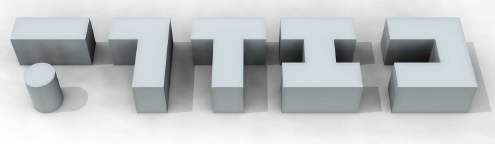
\includegraphics[width=0.95\textwidth]{img/Procedural-Modeling-of-Cities/MassModeling2.png}
  \caption{caption}
  \label{fig:label}
\end{figure}

The next step is to add the roof, from a set of basic roof shapes or general L-Systems.

After that, with the application of the grammar rules in the created mass, it's possible to create complexity to the level that is desired, being able to produce high complex buildings like the one in the following picture.

% subsubsection buildings (end)

\subsubsection{Cities} % (fold)
\label{ssub:Cities1}

The result can be an city like Figure~\ref{fig:bigCity}, with approximately 26000 buildings.

\begin{figure}[htbp]
  \centering
  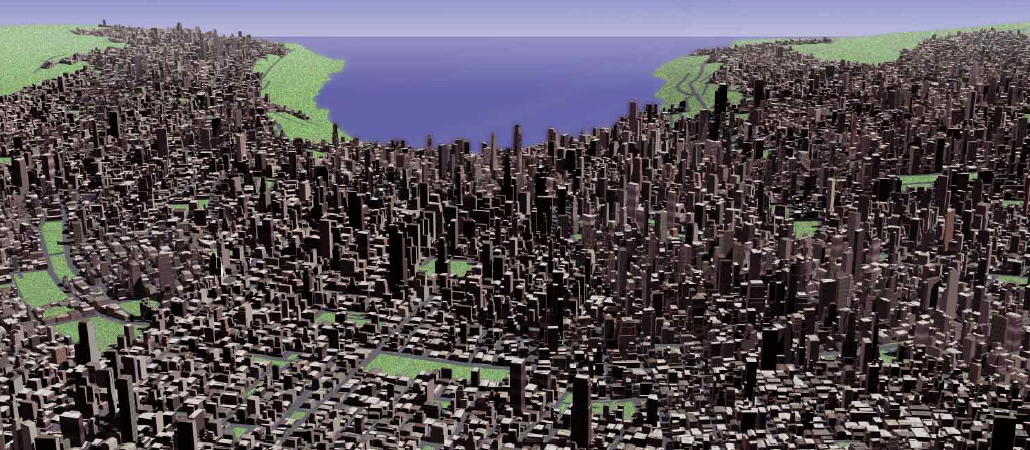
\includegraphics[width=0.95\textwidth]{img/Procedural-Modeling-of-Cities/City.png}
  \caption{City with approximately 26000 buildings.}
  \label{fig:bigCity}
\end{figure}

City Engine results can be imported by Maya, to achieve better results. Like the Figure~\ref{fig:cityMaya}, that represents a ‘virtual’ Manhattan.

\begin{figure}[htbp]
  \centering
  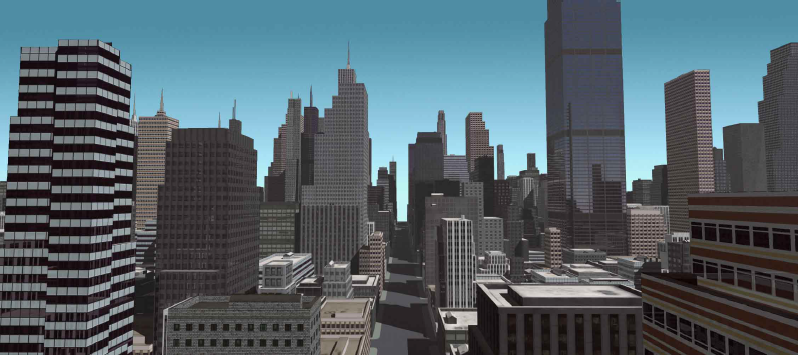
\includegraphics[width=0.95\textwidth]{img/Procedural-Modeling-of-Cities/City_Maya.png}
  \caption{City rendered with Maya.}
  \label{fig:cityMaya}
\end{figure}

% subsubsection subsubsection_name (end)
